\chapter{Community-Led OurPlace Engagements}
The original research path of the OurPlace project can be split into two branches: investigating how the application can be used as a seamless, place-based learning tool within formal education contexts; and how it can be used as a platform for civic learning, with place stakeholders sharing knowledge and values to meet their own agendas. This chapter focuses on engagements which meet the latter, describing an multiyear ethnographic study with a local heritage group, and the engagements which came as a result of it. Some of the work covered by this chapter was peer-reviewed and published at MobileHCI 2018 \citep{Richardson2018}, with the paper being co-authored by Doctors Pradthana Jarusriboonchai, Kyle Montague and Ahmed Kharrufa.

\subsubsection{For clarity}
During the early engagements covered in this chapter, the OurPlace platform was still called `ParkLearn', and lacked the Follow-Up Tasks functionality. Otherwise, the apps were functionally very similar---see Chapter \ref{chap:Design} for more information. The rebranding of ParkLearn to OurPlace occurred in response to findings covered in this chapter.

\section{Creating a Talking Statue using ParkLearn}

Two members (male and female, aged in their 60s) of a local park's volunteer group approached the Parks2026 (discussed in Section \ref{sec:Parks2026}) research group, following engagements unrelated to this project. They had seen the Talking Statues project \citep{Sing2017}, and wanted to produce their own version for their park. This original version used QR codes to launch a mobile-friendly website, where celebrity narrations would inform the user about the history of the statue and the local area. The volunteers wanted to make their own version, built upon an existing monument of a key figure of their park's history. They wanted this `talking statue' to share his story with visitors, encourage them to further explore the park and even to join the volunteer group. However, as the volunteers had very limited technical knowledge and funds, a bespoke digital technology (in the same vein as the original Talking Statues project) seemed inaccessible to them. A physically wired system would have also been too expensive, and would also have interfered with the monument’s status as a listed historical structure. They had hoped that our research group would see this as an opportunity to create a new research project. When this didn't happen, I recognised that the newly expanded ParkLearn app was a viable alternative.

I met with the volunteers at their park, to introduce them to the ParkLearn app and discuss what they would want out of the project. While they were satisfied with the app's functionality, they were most taken by the lack of infrastructure needed by the app, and the potential speed of its deployment: they had previously anticipated the installation to take over a year to develop and deploy, whereas the ParkLearn Activity could be ready almost immediately. Furthermore, they were very surprised by the lack of cost---something which was a major concern, as the volunteer group existed on a shoestring budget. With these reasons in mind, the volunteers decided to create the installation using the app. This was to be the first deployment of ParkLearn `in the wild'.

While the process of creating an Activity can be completed in only a couple of minutes, the talking statue took several weeks to prepare. This was partly down to the need to decide upon and generate content: the volunteers needed to write a script for what the statue should say, and also decide on what else should be included in the Activity. Several drafts were written, balancing the desire to add historical detail with the need to keep the audio recordings short and accessible. The volunteers also considered ways in which they could advertise their volunteer group to interested visitors---as well as inform learners about the park's history, they also wanted to spread awareness of their group's efforts, and how it could be supported. Finally, the volunteers also needed to decide how the Activity should be accessed by visitors. They decided that in order to access the Activity, the user should have to be at the statue in person. This meant that the Activity would have to be set to private, with QR Code scan points provided at the statue itself. Another factor which delayed the deployment was that the volunteers applied for funding from the local council to print Foamex signs, which would be stronger and more weather resistant than laminated paper. They also required permission from the council to feature these signs semi-permanently in the park.

\begin{figure*}
  \centering
  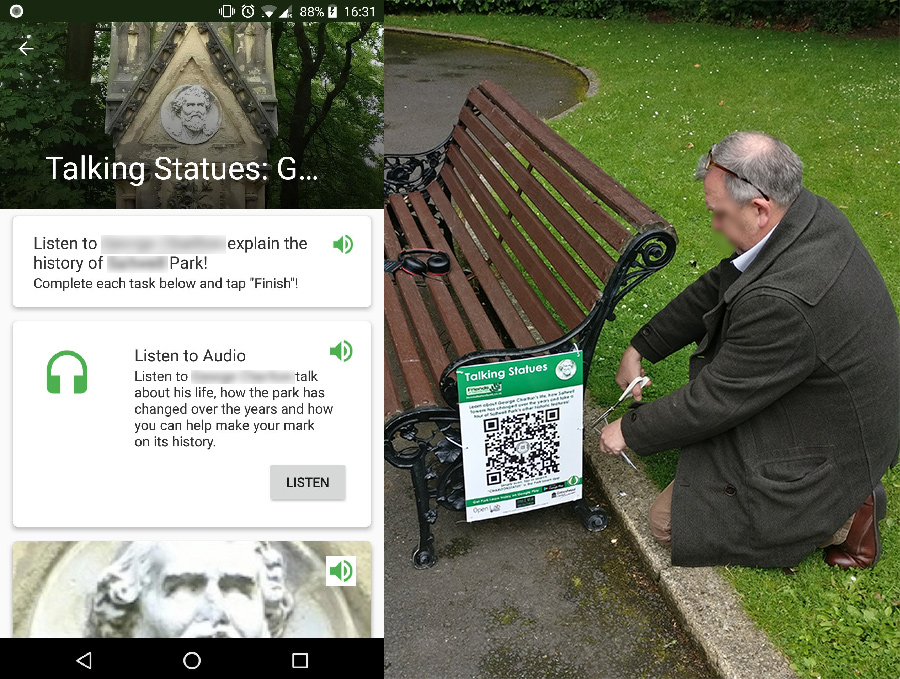
\includegraphics[width=0.9\columnwidth]{images/chapter06/TalkingStatue2.jpg}
  \caption[The ParkLearn `Talking Statue' Activity, and installing the signage ]{Left to right: A) The `Talking Statue' ParkLearn Activity. B) The male park volunteer installing Foamex signs featuring the Activity's QR code.}~\label{fig:TalkingStatueActivity}
\end{figure*}

The final `talking statue' Activity was created at the female volunteer's house, with my help (while both had a base level of digital literacy, neither were hugely comfortable with using new technologies). The Activity featured a narration of the park's history from the perspective of the statue, written and read by the male volunteer. This was recorded directly into the app for a \textit{Listen to Audio} Task (Figure \ref{fig:TalkingStatueActivity}.A). The volunteers were keen for a written transcript of the narration to also be included, so that the Activity would be accessible to those who are hard of hearing. To this end, the speech was transcribed using \textit{Information} Tasks, which also featured historical photos of the park and external links to the volunteer group's website. Finally, the Activity used \textit{Location Hunt} Tasks to guide the learner to the park's eight listed structures (unfortunately as ParkLearn lacked Follow-Up Tasks, no additional content could be unlocked upon arrival).

The Foamex signs were printed with a simple design featuring the Activity's QR code (supplied by the ParkLearn website), and attached to benches near the statue using zip ties (Figure \ref{fig:TalkingStatueActivity}.B). By making the Activity ‘private’ and using these signs, the volunteers could ensure that only people near the statue could launch the Activity. As this meant people would have to be present in the park to use it, they treated the statue as an attraction, something that would raise the profile of the park and encourage people to visit. They printed posters to advertise the project to the surrounding community, and even talked to the local press. 

\begin{figure*}
  \centering
  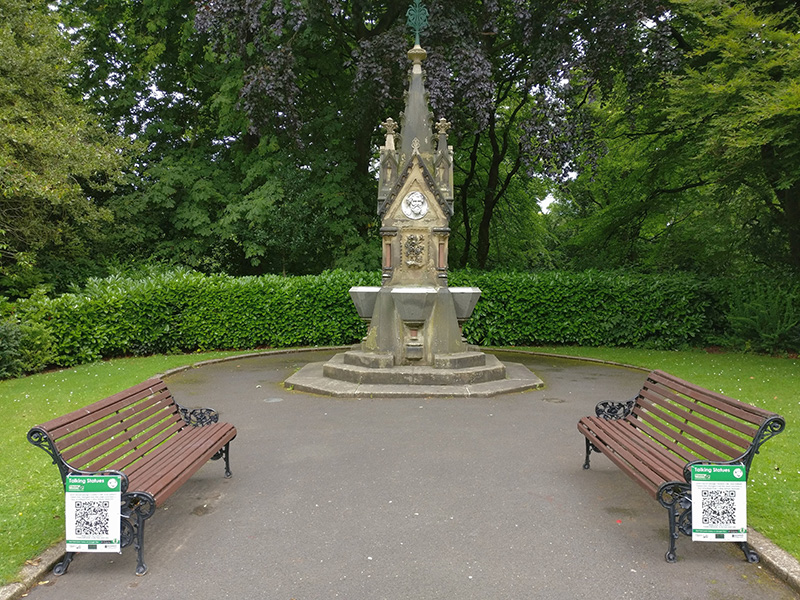
\includegraphics[width=0.9\columnwidth]{images/chapter06/TalkingStatue.jpg}
  \caption[The ParkLearn `Talking Statue' installation]{The final ParkLearn `Talking Statue' installation.}~\label{fig:TalkingStatue}
\end{figure*}

After the launch of the installation, the volunteers were eager for regular updates regarding its usage by park visitors. To facilitate, I updated the ParkLearn website to show the number of times each Activity had been scanned (95 scans in the first 30 days). They were proud of the installation, and demoed it to several volunteer groups from other parks in the area. The signs are still in place over two years later (although one was stolen, and had to be replaced), with around 1200 scans logged.

ParkLearn allowed the volunteers to create a digital, multimedia instalment with minimal interaction or support from the local council (from whom they required permission to put up the scan points). Due to the use of pre-existing technology, the total cost of the installation was around £50 (the cost of producing the signs). The talking statue launched in the same summer in which it was conceived, rather than the original target launch date of the following year. With assistance from the researcher, the actual creation of the Activity took less than an hour.

\section{An Ethnography within the Tyne \& Wear Heritage Forum}

\subsection{An Overview of the TWHF}

\subsection{Engagements and Workshops}

\section{Resulting Interest in and Uptake of OurPlace}

\section{Stakeholder Desires, Requirements and Tensions}

\section{Challenges Encountered}

\section{Summary}